\section{Why these model parameters}
\label{app:choice}

The model has few inputs (Table~\ref{tab:params}), and each was fixed by what the experiment needs: a clean two-level picture in which the prepared state lives in the lowest two levels (the doublet), a transfer time $t^*$ that a finite window can resolve, and a capped core that does not matter for the splitting. Two tables record the choice. Table~\ref{tab:Asweep} sweeps the barrier strength $A$ for one particle, where everything is known; Table~\ref{tab:choice} changes one input at a time for $N=2$ by exact diagonalization and applies two tests to each change. The \emph{overlap} is the weight of the start state in the two lowest levels, and must be at least $\num{ch_ov_min}$; the \emph{cap} test is the relative change of the splitting $\Delta E_2$ when the core cap is doubled, and must be below $\num{ch_cap_max}$. The production point passes both (Table~\ref{tab:choice}).

\begin{table}[ht]
\centering
\footnotesize
\caption{Barrier strength: one particle in $U=A(x^2-1)^2$ ($m=\hbar=1$). $S_0=\frac43\sqrt{2A}$ is the barrier action, $\mut=\sqrt{8A}$ the trap mass (the level spacing $\hbar\omega$ of one valley), $\Delta E$ the splitting of the two lowest levels (finite differences, converged in the grid spacing; the value on the coarse grid $\Delta x=0.125$ is up to $\num{ch_grid_gap}\%$ away), $t^*=\pi/\Delta E$ the time of one complete transfer. $A=\num{A}$ (bold) is the value used in the paper; its $N=2$ value, with the other valley and the pair interaction, is $t_0=\num{tstar0}$ (Table~\ref{tab:params}).}
\label{tab:Asweep}
\begin{tabular}{rccccc}
\toprule
$A$ & barrier action $S_0$ & trap mass $\mut$ & splitting $\Delta E$ & transfer time $t^*=\pi/\Delta E$ & $\Delta E\,/\,\hbar\omega$ \\
\midrule
2 & 2.67 & 4.0 & 0.692 & 4.5 & 0.17 \\
4 & 3.77 & 5.7 & 0.462 & 6.8 & 0.082 \\
6 & 4.62 & 6.9 & 0.297 & 10.6 & 0.043 \\
\textbf{8} & \textbf{5.33} & \textbf{8.0} & \textbf{0.191} & \textbf{16.4} & \textbf{0.024} \\
10 & 5.96 & 8.9 & 0.125 & 25.1 & 0.014 \\
12 & 6.53 & 9.8 & 0.0833 & 37.7 & 0.0085 \\
16 & 7.54 & 11.3 & 0.0389 & 80.8 & 0.0034 \\
\bottomrule
\end{tabular}
\end{table}


A deeper barrier slows the transfer exponentially (Table~\ref{tab:Asweep}). A longer transfer needs a longer window, and the splitting becomes a smaller fraction of the level spacing $\hbar\omega$.

\begin{table}[ht]
\centering
\footnotesize
\setlength{\tabcolsep}{4pt}
\caption{Why these inputs: $N=2$ by exact diagonalization on a $28\times18$ grid, one input changed at a time from the production point ($A=8$, $\epsilon=2$, $\sigma=0.18$, $\omega_y^2=2$, $C_0=0.15$, $V_{\rm cap}=100$). $c^*$: tilt at which the ground state has $\langle\Op\rangle=\frac12$; $\Delta E_2$: splitting of the two lowest levels; overlap: weight of the start state in those two levels (need $\ge\num{ch_ov_min}$); cap: relative change of $\Delta E_2$ when the core cap is doubled (need $<\num{ch_cap_max}$).}
\label{tab:choice}
\begin{tabular}{L{3.9cm}ccccc}
\toprule
changed input & tilt $c^*$ & $\Delta E_2$ & overlap & cap & verdict \\
\midrule
production point & 0.406 & 0.1901 & 0.979 & 0.007 & pass \\
barrier $A=4$ & 0.396 & 0.4287 & 0.871 & 0.078 & \textbf{fail: overlap} \\
$A=6$ & 0.393 & 0.2839 & 0.941 & 0.067 & pass \\
$A=10$ & 0.421 & 0.1278 & 0.993 & 0.162 & \textbf{fail: cap} \\
$A=12$ & 0.435 & 0.0866 & 0.997 & 0.415 & \textbf{fail: cap} \\
range $\sigma=0.25$ / $0.35$ & 0.572 / 0.568 & 0.1835 / 0.1856 & 0.980 / 0.980 & 0.012 / 0.016 & pass \\
$\sigma=0.5$ & 0.898 & 0.1378 & 0.461 & 0.048 & \textbf{fail: overlap} \\
depth $\epsilon=0.5,1,2,4,8$ & 0.391--0.411 & 0.1901--0.1904 & 0.979 & 0.004--0.008 & pass \\
transverse $\omega_y^2=0.5$ / $8$ & 0.245 / 0.662 & 0.1822 / 0.2025 & 0.980 / 0.974 & 0.019 / 0.061 & pass \\
offset $C_0=0$ & 0.421 & 0.1532 & 0.738 & 0.262 & \textbf{fail: both} \\
$C_0=0.05$ & 0.408 & 0.1657 & 0.877 & 0.188 & \textbf{fail: both} \\
$C_0=0.30$ & 0.409 & 0.1972 & 0.990 & 0.073 & pass \\
cap $V_{\rm cap}=25$ / $400$ & 0.237 / 0.490 & 0.1901 / 0.1889 & 0.978 / 0.979 & 0.095 / 0.016 & pass \\
\bottomrule
\end{tabular}
\end{table}


The table gives the following reading.
\begin{itemize}
\item \textbf{$A=\num{ch_A_deep}$ is the deepest barrier that passes.} At $A=4$ the start state leaks out of the two levels; $A=6$ passes. At $A=10$ and $12$ the capped core shifts the splitting by far more than the limit: the splitting is exponentially small, so the same perturbation of the core is a larger fraction of it.
\item \textbf{Range $\sigma$.} $\sigma=0.25$ and $0.35$ change nothing that matters, while $\sigma=0.5$ breaks the picture: the pair is no longer confined to the two lowest levels.
\item \textbf{Depth $\epsilon$ and transverse stiffness $\omega_y^2$.} Over $\epsilon=0.5,\dots,8$ the splitting and the overlap barely change; only the resonant tilt moves. Both $\omega_y^2=0.5$ and $8$ pass.
\item \textbf{Offsets $C_0$.} Without a sufficient offset between the tilts of the particles the pair fails both tests ($C_0=0$ and $0.05$); $C_0=0.15$ and $0.30$ pass. This is consistent with Remark~\ref{rem:symm}: nearly symmetric preparations behave differently from the generic case.
\item \textbf{Cap $V_{\rm cap}$.} At $V_{\rm cap}=25$ the cap test fails narrowly; $100$ and $400$ pass, so the cap used is inert for the quantities in this paper.
\end{itemize}
The one-particle splitting (Table~\ref{tab:Asweep}) is for a single particle without the transverse direction or a partner; the switching time $t_0$ of the main runs (Table~\ref{tab:params}) is computed from the $N=2$ splitting on the production grid.

\paragraph{Does the choice carry over to larger $N$?}
The tests of Table~\ref{tab:choice} are for $N=2$. Table~\ref{tab:Ascan} repeats the overlap test at $N=3$ and $N=4$ in the $k=12$ basis, finding the resonant tilt again for each $A$ (static diagonalization; no propagation). At $N=3$ the deeper barriers give a clean doublet while $A=6$ does not and $A=4$ has none at all. Combined with $N=2$, where $A=6$ and $8$ pass the overlap test and $A\ge10$ fail the cap test, $A=\num{A}$ is the only tested value that passes the $N=2$ tests and the $N=3$ overlap test, which makes it a consistent choice. It is not shown to be the best one: the cap test was not repeated at $N=3$, and the overlap at $N=3$ is as good at $A=10$ and $12$.

\begin{table}[ht]
\centering
\footnotesize
\caption{Does the barrier chosen at $N=2$ carry over? Static scan at $N=3$ and $4$ in the $k=12$ mode basis (no propagation): for each $A$ the resonant tilt is found again, and the correlated start is prepared as in the main runs. $c^*$: tilt; $\Delta E$: splitting of the doublet that the doublet test selects; overlap: weight of the start in that doublet (need $\ge\num{ch_ov_min}$). A row marked \emph{no doublet} has no pair of levels that passes the doublet test at the resonance found. The cap test of Table~\ref{tab:choice} was not repeated for $N>2$.}
\label{tab:Ascan}
\begin{tabular}{rrcccc}
\toprule
$N$ & $A$ & $c^*$ & $\Delta E$ & overlap & verdict \\
\midrule
3 & 4 & 1.24 & 0.314 & 0.823 & \textbf{fail: no doublet} \\
3 & 6 & 1.42 & 0.108 & 0.598 & \textbf{fail: overlap} \\
\textbf{3} & \textbf{8} & \textbf{1.47} & \textbf{0.191} & \textbf{0.935} & pass \\
3 & 10 & 1.48 & 0.125 & 0.960 & pass \\
3 & 12 & 1.47 & 0.083 & 0.956 & pass \\
\midrule
4 & 6 & 2.22 & 0.092 & 0.382 & \textbf{fail: no doublet} \\
\textbf{4} & \textbf{8} & \textbf{2.28} & \textbf{0.051} & \textbf{0.409} & \textbf{fail: no doublet} \\
4 & 10 & 2.26 & 0.105 & 0.813 & \textbf{fail: overlap} \\
4 & 12 & 2.26 & 0.089 & 0.760 & \textbf{fail: overlap} \\
\bottomrule
\end{tabular}
\end{table}


At $N=4$ no tested barrier passes at $k=12$, but the overlap rises with depth (Table~\ref{tab:Ascan}). The failure of the doublet test at $N=4$, $k=12$ reported in Section~\ref{sec:measured} is therefore in part a property of this working point and this basis, not of $N$ alone. A deeper barrier lengthens the movie and, at the grid resolution used, makes the capped core matter more, so it is not a free improvement. What the data support is limited: $A=\num{A}$ gives a clean two-level picture at $N=2$ and $3$, the resonant tilt grows with $N$ (Table~\ref{tab:start}), and whether another barrier, with a finer grid, keeps a doublet at larger $N$ and how the entropies at $N\ge4$ would then change has not been measured. The offsets $C_0$ and the other inputs were likewise tested at $N=2$ only. All entropy results of the paper are for this working point.

\section{Proofs and exact statements}
\label{app:proofs}

Throughout, $\psi$ is a pure state of $N$ particles with local dimension $d$, $S_A$ is the von Neumann entropy in bits of the reduced state on a set $A$ of $a$ particles, and $S_i=S_{\{i\}}$.

\subsection{Cuts and tensor networks}

\begin{lem}[Rank and size of a cut]\label{lem:cap}
(a) The Schmidt rank of $\psi$ across $A\,|\,A^c$ is at least $2^{S_A}$ and at most $d^{\min(a,N-a)}$; hence $S_A\le\min(a,N-a)\log_2d$. (b) $S_A\le\sum_{i\in A}S_i$.
\end{lem}
\begin{proof}
The entropy of a distribution on $r$ outcomes is at most $\log_2r$, so $S_A\le\log_2\mathrm{rank}\rho_A$, and $\mathrm{rank}\rho_A\le\dim\mathcal H_A=d^a$; the same holds for $A^c$ because $\rho_A$ and $\rho_{A^c}$ have the same spectrum. (b) is subadditivity.
\end{proof}
A tensor network that represents $\psi$ exactly and has a bond that separates $A$ from $A^c$ has bond dimension at least the Schmidt rank across that cut; with (a) this is Proposition~\ref{prop:tn}(a)--(b).

\begin{lem}[Pivot]\label{lem:pivot}
In a tree tensor network on $N\ge4$ particles in which every node has degree at most three (physical legs counted), some bond has between $\lceil N/3\rceil$ and $\lfloor N/2\rfloor$ particles on its smaller side.
\end{lem}
\begin{proof}
Orient each bond towards the side with more particles (ties arbitrarily). A finite tree has a node $v$ with all incident bonds pointing at it, so each of the at most three branches at $v$ holds at most $N/2$ particles. The branches partition the $N$ particles, so the heaviest holds at least $N/3$;
it is a bond rather than a physical leg once $N\ge4$. Its smaller side is the complementary part, with between $\lceil N/3\rceil$ and $\lfloor N/2\rfloor$ particles.
\end{proof}
The bound is attained, for example, by a tree whose central node has three equal branches. A matrix-product state and any balanced binary tree qualify. Hence no layout avoids a cut with a number of particles of order $N$ on both sides, which is why $\Sperp$ is the quantity every such layout pays.

\begin{lem}[Size-averaged cut profile]\label{lem:chord}
Let $s(a)$ be the entropy of $\psi$ averaged over all subsets of size $a$. Then $s(0)=s(N)=0$, $s(a)=s(N-a)$, $s(a)$ is concave in $a$, and $s(a)/a$ is non-increasing; in particular $s(a)\ge\frac{a}{\lfloor N/2\rfloor}s(\lfloor N/2\rfloor)$ for $a\le\lfloor N/2\rfloor$.
\end{lem}
\begin{proof}
$s(0)=s(N)=0$ and the symmetry are purity. For disjoint $C$ and distinct $i,j\notin C$, strong subadditivity gives $S_{C\cup\{i,j\}}+S_C\le S_{C\cup\{i\}}+S_{C\cup\{j\}}$; averaging over all $C$ of size $a-1$ and over $i\ne j$ gives $s(a+1)+s(a-1)\le2s(a)$, i.e. concavity. Concavity with $s(0)=0$ gives $s(a)/a$ non-increasing, and the last statement
follows by the chord inequality.
\end{proof}
Consequently a cut at a fraction $a/N$ of the system carries at least $2a/N$ of the central value, which is the sense in which the bond profile of a matrix-product state is concave and the central bond is the expensive one. The lemma concerns averages over subsets and needs no symmetry; for a particular subset the entropy can deviate (Table~\ref{tab:measured}).

\begin{rem}[Symmetric preparations are cheap]\label{rem:symm}
If $\psi$ is invariant under permutations of the particles, it lies in the symmetric subspace, of dimension $\binom{N+d-1}{d-1}=O(N^{d-1})$ at fixed $d$, so every cut has Schmidt rank at most $\binom{a+d-1}{d-1}$ and $S_A\le(d-1)\log_2N+O(1)$. A growth that is faster than logarithmic therefore needs the permutation symmetry to be broken,
here by the offsets $c_i$ and by the choice of which particle starts in the right valley.
\end{rem}

\subsection{The correlation graph}

\begin{prop}[Pairwise statements]\label{prop:graph}\stE{}
Let $I_{ij}=S_i+S_j-S_{ij}$.\\
(a) For a pure state $S_A=\tfrac12I(A\!:\!A^c)$. (b) For $|A|=2$, $S_A=S_i+S_j-I_{ij}$. (c) For every spanning tree $\tau$ on $A$, $S_A\le\sum_{i\in A}S_i-\sum_{(ij)\in\tau}I_{ij}$. (d) For $N=3$ and every fixed $t$, $I_{ij}+I_{il}=2S_i$, so $C(\{i\})=S_i$.\\
(e) $C(A)$ is neither an upper nor a lower bound on $S_A$ for general states: a GHZ state of $N\ge4$ qubits has $S_A=1$ and $I_{ij}=1$, so $C(A)=a(N-a)/2>S_A$ for $a\ge2$; a Haar-random state of $N$ qudits with $d^{N-2}\gg d^{2}$ has $I_{ij}\to0$ and $S_A\to\min(a,N-a)\log_2d$, so $C(A)\ll S_A$.
\end{prop}
\begin{proof}
(a) For pure $AA^c$, $S_{A^c}=S_A$ and $S_{AA^c}=0$. (b) is the definition. (c) Remove a leaf $\ell$ of $\tau$ with neighbor $p\in A$. Then $S_A=S_{A\setminus\ell}+S_\ell-I(\ell\!:\!A\setminus\ell)$ and $I(\ell\!:\!A\setminus\ell)\ge I_{\ell p}$ by monotonicity of mutual information under partial trace; induct on $|A|$.
(d) For three parties in a pure state $S_{jl}=S_i$ and so on, hence $I_{ij}+I_{il}=2S_i+S_j+S_l-S_{ij}-S_{il}=2S_i$. (e) follows from the stated examples. With time-maximal weights $w_{ij}=\max_tI_{ij}(t)$, (d) holds only at fixed $t$, which is why the graph of Section~\ref{sec:graph} overcounts at $N=3$.
\end{proof}
Monogamy of mutual information, $I(X\!:\!YZ)\ge I(X\!:\!Y)+I(X\!:\!Z)$, would give $\sum_jI_{ij}\le2S_i$ and $C\le S$; it holds for holographic states~\cite{hayden2013} but not in general (a GHZ state, which is a stabilizer state, violates it). The measured ratio $\sum_jI_{ij}/2S_i$ is close to one (Section~\ref{sec:graph}), the boundary of monogamy, where the sharing law is exact.

\subsection{The conditional reduction}

\begin{proof}[Proof of Proposition~\ref{prop:cond}]
Write $|\psi(t)\rangle=\sum_{m=1}^{M+2}c_m e^{-iE_mt}|m\rangle+|\eta(t)\rangle$ with $|m\rangle$ the eigenstates spanning $\mathcal S$ and $\|\eta\|\le\delta$. Then $f(t)=\langle\psi|\Op|\psi\rangle=\sum_{m,n}c_m^\ast c_n O_{mn}e^{i(E_m-E_n)t}+r(t)$ with $|r(t)|\le2\|\Op\|\delta+\|\Op\|\delta^2\le3N\delta$ for $\delta\le1$, since $\|\Op\|=N$. Real parts of the $m\ne n$ terms pair into $\binom{M+2}2$ cosines and the diagonal terms are constants, so at most $(M+2)(M+3)/2$ terms. For the rank statement let $|\psi\rangle=a|F\rangle+\sum_ib_i|I_i\rangle$ with $|F\rangle=\bigotimes_j|L_j\rangle$ and $|I_i\rangle=|R_i\rangle\bigotimes_{j\ne i}|L_j\rangle$ product states. Across a cut $A\,|\,A^c$ separate the sum into the terms with $i\in A$ and $i\in A^c$: $|\psi\rangle=|\alpha\rangle_A|L\rangle_{A^c}+|L\rangle_A|\beta\rangle_{A^c}$ with $|\alpha\rangle_A=a|L\rangle_A+\sum_{i\in A}b_i|R_i\rangle\bigotimes_{j\in A\setminus i}|L_j\rangle$ and $|\beta\rangle_{A^c}=\sum_{i\in A^c}b_i|R_i\rangle\bigotimes_{j\in A^c\setminus i}|L_j\rangle$. That is a sum of two product vectors, so the Schmidt rank is at most two and $S_A\le1$ bit. For states of bond dimension $\chi_0$ in a common ordering, the span of $M+2$ states has bond dimension at most $(M+2)\chi_0$ (bond dimensions add under superposition).
\end{proof}
The ideal case is the product-orbital limit $M=0$. It is not what the correlated start is: the correlation hole of particles that share a valley is not a product state, and its entropy is the static entropy of Section~\ref{sec:static-entropy}.

\subsection{The quantum edge}

\begin{proof}[Derivation of Eq.~\eqref{eq:muqub} and of its two properties]
The query count $\lceil\lambda\Tobs+\ln(1/\varepsilon)\rceil$ times $C_{\rm sel}$ is at most $\BT$ iff $\lambda\Tobs\le X$ with $X=\BT/C_{\rm sel}-\ln(1/\varepsilon)$. Inserting Eq.~\eqref{eq:Tobs}, $\lambda\,g_N t_0e^{2(\mut-\mut_0)/3}(\mut_0/\mut)^{1/2}\le X$; taking logarithms and solving for $\mut$ gives Eq.~\eqref{eq:muqub}. Differentiating with respect to $\ln\BT$ at fixed $N$ gives $\partial\mutq/\partial\ln\BT\simeq\tfrac32$ to leading order
(the $\mut$-dependence of the last term and of $\ln X$ is subleading). For $\lambda\simeq\frac12N^2\lambda_W$, $\mutq(N)-\mutq(N_0)\simeq-\tfrac32\ln(N^2/N_0^2)=-3\ln(N/N_0)$.
\end{proof}

\begin{prop}[Barrier action of a recoil-scaled optical lattice]\label{prop:lattice}\stE{}
In the lattice $V(x)=sE_r\sin^2(kx)$, $E_r=\hbar^2k^2/2m$, the action under one barrier at zero energy is
\[S_0=\frac1\hbar\int_0^{\pi/k}\sqrt{2m\,sE_r}\,\sin(kx)\,dx=2\sqrt s\]
for every species, so $\mut=\tfrac32S_0=3\sqrt s$.
\end{prop}
\begin{proof}
$\sqrt{2mE_r}/\hbar=k$ and $\int_0^{\pi/k}\sin(kx)\,dx=2/k$. The zero-point energy is neglected.
\end{proof}
This is the exponent of the standard deep-lattice tunneling matrix element; it concerns the single-particle action only, since the pair-interaction cost of Appendix~\ref{app:quantum} depends on the species. For the trap of Eq.~\eqref{eq:HN}, $S_0=\frac43\sqrt{2mA}\,a/\hbar$ with $A=\num{A}$, $m=1$, $a=1$ gives $S_0=\num{Szero}$, $\mut=\num{mut0}$.

\section{Numerical details}
\label{app:numerics}

\paragraph{Bases and starts.}
The grid has $\num{nx}\times\num{ny}$ cells over $[-L_x,L_x]\times[-L_y,L_y]$ with $L_x=\num{Lx}$, $L_y=\num{Ly}$ ($\Delta x=\num{dx}$, $\Delta y=\num{dy}$) and the core of the pair potential smeared over $\num{smear}$. The mode basis keeps the $k=12,16,20$ lowest eigenstates of one particle;
product orbitals are the valley-localized combinations of these. The correlated start is the ground state of $\hat H_N+W\sum_iP_i^{\rm wrong}$ with $W=\num{Wpen}$ and the penalty on the wrong side of each particle. The state is propagated with Chebyshev polynomials of $\hat H_N$ and recorded every $\Delta t=\num{dtsnap}$ over $0\le t\le T=\num{Tprot}$ ($\num{nsnap}$ snapshots), the same for every $N$ and $k$; entropies are computed at each snapshot for every subset with $|A|\le N/2$.

\paragraph{Resonance and window.}
For each $N$ and $k$ the tilt $c^*$ is the value at which the ground state of the mode-basis Hamiltonian has $\langle\Op\rangle$ closest to one half; it shifts with $k$ (Table~\ref{tab:start}). The weight $\Theta(0)=\tfrac12$ of the grid column on the barrier top is a convention (see below). Every entropy in the paper is a maximum over the same window $[0,T]$ with $T=\num{Tprot}$ and the same spacing $\Delta t=\num{dtsnap}$, for every $N$ and $k$; a shorter window is a cut of the stored series, never a different run. The choice matters (Table~\ref{tab:protocol}). \emph{Window:} the central bond keeps creeping up at $N=2$, and at $N=4$ a short window misses the maximum; at $N=5$ and $N=6$ the central bond is still rising slowly at the end of the window (Table~\ref{tab:measured}), so these entropies are lower bounds on their windowless values. \emph{Spacing:} the maximum over snapshots is a lower bound that rises as the spacing shrinks, but at the spacing used it is within about a hundredth of a bit of the finest spacing tried (Table~\ref{tab:protocol}). A cut whose maximum is at the last snapshot is likewise a lower bound on its entropy; none of the cuts of any run peaks at the last snapshot.

\begin{table}[ht]
\centering
\footnotesize
\caption{Sampling sensitivity of the entropy maxima (bits; correlated start, $k=12$). \emph{Window} (upper block): one stored series of the protocol ($T=\num{Tprot}$, spacing $\num{dtsnap}$) cut to a shorter window afterwards: central bond $S_{\rm cen}$ and worst balanced cut $\Smax$ (equal at $N=2$, where there is one cut). \emph{Spacing} (lower block): the same state and window with another snapshot spacing $\Delta t$; the maximum is taken over the snapshots.}
\label{tab:protocol}
\begin{tabular}{lcccc}
\toprule
 & \multicolumn{3}{c}{window: $S_{\rm cen}$ / $\Smax$} \\
\cmidrule(lr){2-4}
$N$ & $T\le60$ & $T\le120$ & $T\le200$ & \\
\midrule
2 & 0.869 / 0.869 & 0.879 / 0.879 & 0.905 / 0.905 & \\
3 & 1.297 / 1.367 & 1.298 / 1.367 & 1.298 / 1.367 & \\
4 & 2.264 / 2.360 & 2.335 / 2.542 & 2.335 / 2.542 & \\
\midrule
spacing at $T=\num{Tprot}$ & $\Delta t=0.5$ & $\Delta t=1$ & $\Delta t=2$ & $\Delta t=4$ \\
\midrule
$N=3$, max one-particle entropy & 1.382 & 1.367 & 1.367 & 1.367 \\
$N=3$, $S_{\rm cen}$ & 1.298 & 1.298 & 1.297 & 1.297 \\
$N=4$, $S_{\rm cen}$ & 2.335 & 2.335 & 2.335 & 2.326 \\
\bottomrule
\end{tabular}
\end{table}


\paragraph{The convention $\Theta(0)=\tfrac12$.}
The grid has one column exactly on the barrier top, $x=0$. Counting it as left would treat the two valleys differently by the weight of that column (under one per cent of a symmetric ground state), so every simulation in this paper gives it weight $\tfrac12$. The alternative convention was also run and changes little: over all correlated-start runs the central-bond entropy moves by at most $\num{th_dS_cen_max}$ bit, the splittings and every product-start entropy are unchanged (the Hamiltonian does not contain $\Theta$), and the first failing $N$ of every route in Table~\ref{tab:walls} is the same. The convention is a bookkeeping choice, not a physical effect at the resolution of this paper.

\paragraph{The switching time $t_0$.}
The cost model of Section~\ref{sec:quantum} takes $t_0=\num{tstar0_2}$, the switching time $\pi/\dE_2$ of the two-particle problem on the position grid, and Section~\ref{sec:model} quotes it. It depends on where the tilt sits, because $\dE_2$ rises with $c$ near the resonance: at the exact resonance of the present convention it is $\num{t0_dpct}\%$ below the quoted value. We keep the quoted value because it is the number the cost model was evaluated with and the choice does not matter here: the transfer time enters the T-gate count linearly and the mass edge through $\tfrac32\ln t_0$ (Eq.~\eqref{eq:muqub}), so using the resonant value moves the edge by $+\num{t0_edge_shift}$ in $\mut$, small against its fall with $N$ (Table~\ref{tab:quantum}). The mode-basis runs have their own resonance tilts (Table~\ref{tab:start}), so $t_0$ is a statement about the grid, not about their $\dE_N$.

\paragraph{Basis dependence.}
Table~\ref{tab:k} and Fig.~\ref{fig:kconv} give the central entropy and the numerical Schmidt rank for $k=12,16,20$; Table~\ref{tab:start} the two-level picture and the per-$k$ resonance tilts.

\begin{table}[ht]
\centering
\footnotesize
\caption{Basis dependence of the central-cut entropy (bits, correlated start) and of the numerical Schmidt rank $\chi(10^{-3})$ of that bond. Resonance tilts differ with $k$. }
\label{tab:k}
\begin{tabular}{rcccccc}
\toprule
 & \multicolumn{3}{c}{$S$ (bits)} & \multicolumn{3}{c}{$\chi(10^{-3})$} \\
\cmidrule(lr){2-4}\cmidrule(lr){5-7}
$N$ & $k=12$ & $16$ & $20$ & $k=12$ & $16$ & $20$ \\
\midrule
2 & 0.90 & 0.87 & 0.87 & 7 & 7 & 8 \\
3 & 1.30 & 1.27 & 1.27 & 10 & 11 & 11 \\
4 & 2.33 & 2.11 & 1.92 & 38 & 44 & 47 \\
5 & 2.72 & 2.59 & 2.61 & 74 & 105 & 118 \\
6 & 3.26 & -- & -- & 325 & -- & -- \\
\bottomrule
\end{tabular}
\end{table}


\begin{figure}[ht]
\centering
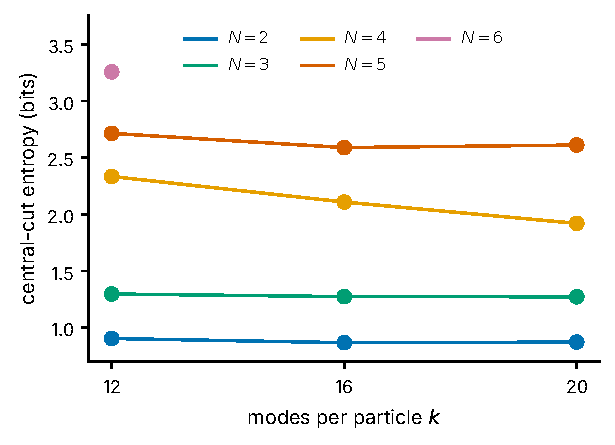
\includegraphics[width=0.6\textwidth]{figures/fig_kconv.pdf}
\caption{Central-cut entropy against the number of modes per particle (correlated start).}
\label{fig:kconv}
\end{figure}

\paragraph{Checks.} The machinery was tested on one-particle problems with known answers (Table~\ref{tab:checks}). The closed form of $\Gamma_\infty$ quoted in Section~\ref{sec:mc} was checked against the numerically summed column of the kinetic operator for $M=64,\dots,65536$ in one dimension; the fitted exponent against $M$ is $\num{p_UV}$.

\begin{table}[ht]
\centering
\footnotesize
\caption{Checks of the numerical machinery on one-particle problems with known answers.}
\label{tab:checks}
\begin{tabular}{L{6.8cm}ccc}
\toprule
Check & computed & reference & relative difference \\
\midrule
Real-time propagation, weak barrier ($A=1$): splitting & 0.791910 & 0.791776 & $\ensuremath{1.7\times10^{-4}}$ \\
Instanton formula against exact diagonalization, $A=8$ & 0.2010 & 0.1913 & 5.0\% \\
\bottomrule
\end{tabular}
\end{table}


\paragraph{Data.} Every number in the text and tables and every figure is generated from stored run logs and time series; entropies, correlation graphs and the extrapolation are derived from them without hand-entered values.

\section{The spectrum of the start: methods, table and checks}
\label{app:static}

This appendix holds everything behind Section~\ref{sec:static}: the method, one table of every case computed (Table~\ref{tab:start}), the structural checks and the remarks on what cannot be established. Nothing here is propagated in time.

\paragraph{What was computed.} For each $(N,k)$ the resonance tilt $c^\ast$ was found as for the main runs (the ground state has $\langle\Op\rangle=\frac12$), the lowest eigenlevels of $\hat H_N$ in the $k$-mode basis were computed (dense diagonalization when $k^N\le8000$, thick-restart Lanczos (ARPACK) otherwise, with $40$ levels, doubled to $80$ and $160$ until the coverage reaches $0.99$ or the memory limit), and the weight $|\langle\text{level}|\text{start}\rangle|^2$ of the correlated start on each was stored with the energy and the multiplicity ($N=5$, $k=24$ has a Lanczos list only). Runs at $k=6,8$ are not used: the six-mode basis crowds the all-left state into too few modes, and their energies are artefacts. Where the coverage stays below $0.99$ the weight $B_2$ of the pair is a lower bound, within $1-\text{coverage}$ of its value (the unresolved levels lie higher in energy). Levels closer than $10^{-6}$ are merged and their weights added.

\paragraph{The pair, and the gated pair.} The pair is the two levels of largest weight in the start, with $J=(E_b-E_a)/2$ and total weight $B_2$; the three distance classes of Table~\ref{tab:start} are measured from the nearer level of the pair. The \emph{gated pair} of Section~\ref{sec:measured} is a different object: the pair of low levels of smallest splitting $\Delta E$ that passes the doublet gates (mixed by $\hat O$, one particle apart in $\langle\hat O\rangle$). It is selected by its splitting, not by its weight, so it need not be the pair that carries the weight, and for $N\ge4$ it is not; where the two differ, the pair is the reading that measures how few-level the start is. A clean gated pair also gives the ratio $g_N=\Delta E_2/\Delta E_N$ of Eq.~\eqref{eq:Tobs}.

\begin{table}[ht]
\centering
\footnotesize
\setlength{\tabcolsep}{3.2pt}
\caption{The correlated start in the eigenbasis of $\hat H$, every case computed (method in the text of this appendix). $c^*$: resonance tilt of the mode basis; coverage: weight of the start on the computed levels. \emph{Pair}: the two levels of largest weight, their splitting $2J$ and total weight $B_2$. \emph{Outside the pair}: the weight on the other levels by distance to the nearer level of the pair (within $J$, $1$--$3J$, beyond $3J$); the remainder $1-B_2-\text{sum}$ is on levels not computed. \emph{Gated pair}: the pair of low levels of smallest splitting $\Delta E$ that passes the doublet gates, the weight of the start on it, and whether it is a clean doublet (with the ratio $g_N=\Delta E_2/\Delta E_N$ of Eq.~\eqref{eq:Tobs}, $\Delta E_2$ the grid value of Table~\ref{tab:params}); it is selected by splitting, not by weight, so it can differ from the pair. Rows marked $^\ast$ are Lanczos lists only; $k=6,8$ are omitted (artefacts of the small basis).}
\label{tab:start}
\begin{tabular}{rrcccccccccc}
\toprule
 & & & & \multicolumn{2}{c}{pair} & \multicolumn{3}{c}{outside the pair} & \multicolumn{3}{c}{gated pair} \\ \cmidrule(lr){5-6}\cmidrule(lr){7-9}\cmidrule(lr){10-12}
$N$ & $k$ & $c^*$ & coverage & $2J$ & $B_2$ & $<J$ & $1$--$3J$ & $\ge3J$ & $\Delta E$ & weight & clean / $g_N$ \\
\midrule
2 & 12 & 0.70 & 1.000 & 0.180 & 0.976 & 0.000 & 0.014 & 0.010 & 0.180 & 0.98 & yes / 1.06 \\
2 & 16 & 0.70 & 1.000 & 0.185 & 0.976 & 0.000 & 0.011 & 0.012 & 0.185 & 0.98 & yes / 1.03 \\
2 & 20 & 0.70 & 1.000 & 0.192 & 0.978 & 0.000 & 0.010 & 0.013 & 0.192 & 0.98 & yes / 0.99 \\
\addlinespace[2pt]
3 & 12 & 1.46 & 1.000 & 0.189 & 0.938 & 0.000 & 0.044 & 0.017 & 0.189 & 0.94 & yes / 1.01 \\
3 & 16 & 1.36 & 1.000 & 0.191 & 0.952 & 0.000 & 0.018 & 0.030 & 0.191 & 0.95 & yes / 1.00 \\
3 & 20 & 1.31 & 1.000 & 0.193 & 0.955 & 0.000 & 0.017 & 0.028 & 0.193 & 0.96 & yes / 0.98 \\
\addlinespace[2pt]
4 & 12 & 2.26 & 0.993 & 0.184 & 0.668 & 0.085 & 0.213 & 0.027 & 0.052 & 0.46 & no \\
4 & 16 & 2.14 & 0.985 & 0.225 & 0.845 & 0.001 & 0.114 & 0.026 & 0.104 & 0.34 & no \\
4 & 20 & 2.02 & 0.986 & 0.218 & 0.906 & 0.000 & 0.056 & 0.024 & 0.218 & 0.91 & yes / 0.87 \\
4 & 24 & 1.94 & 0.975 & 0.220 & 0.921 & 0.000 & 0.042 & 0.012 & -- & -- & -- \\
4 & 28 & 1.87 & 0.977 & 0.220 & 0.931 & 0.000 & 0.018 & 0.028 & -- & -- & -- \\
4 & 32 & 1.82 & 0.976 & 0.221 & 0.934 & 0.000 & 0.018 & 0.024 & -- & -- & -- \\
\addlinespace[2pt]
5 & 12 & 2.92 & 0.971 & 0.362 & 0.683 & 0.268 & 0.016 & 0.004 & 0.152 & 0.35 & no \\
5 & 16 & 2.72 & 0.942 & 0.229 & 0.780 & 0.002 & 0.151 & 0.010 & 0.107 & 0.39 & no \\
5 & 20 & 2.62 & 0.943 & 0.233 & 0.812 & 0.007 & 0.114 & 0.010 & 0.105 & 0.39 & no \\
5 & 24$^\ast$ & 2.57 & 0.918 & 0.251 & 0.836 & 0.005 & 0.077 & 0.000 & -- & -- & -- \\
\addlinespace[2pt]
6 & 12 & 3.66 & 0.936 & 0.437 & 0.729 & 0.194 & 0.013 & 0.000 & 0.173 & 0.31 & no \\
\bottomrule
\end{tabular}
\end{table}


\paragraph{Reading the table.} At $N=2,3$ the two readings coincide and the pair carries almost everything. At $N=4$ the weight of the pair converges with the basis; the small-basis rows are a basis artefact, and the gated pair passes its gates only at one basis size. At $N=5$ neither the weight nor the coverage is converged, and the $k=12$ rows are dominated by levels within $J$ of the pair that vanish at larger $k$; at $N=6$ only one unconverged basis exists. The weight outside the pair that grows with $N$ is the $1$--$3J$ column; the far column is small and does not grow. Where a clean doublet exists, $g_N$ lies close to one, which supports carrying $g_N=1$ in the quantum price.

\paragraph{Reflection symmetry, sector exclusion, label fragmentation.} The reflection $R$ ($y_i\to-y_i$ for all particles) is built in the mode basis as $\prod_iP^\top R_{\rm grid}P$; the one-body parity closure of the truncated modes is about $0.05$, so eigenstate parities are near, not exactly, $\pm1$, and the small odd weights in Fig.~\ref{fig:parity} are leakage of the basis. The start is even to within this leakage ($\langle R\rangle>0.999$ at $N=3,4$). Every level of non-negligible weight is even; the levels between the two members of the pair carry no weight and are odd, so they are not a hidden manifold of transfer states. The right-valley occupation $\langle n_i\rangle$ of particle $i$ is the expectation of the one-particle valley indicator (Table~\ref{tab:levels}): the pair is carried mainly by particle $0$. The first even level with two particles on the right (sector exclusion) is far from the pair at $N=3$ and absent from the computed levels at $N=4$ (Fig.~\ref{fig:parity}). The first levels in which particle $1$ or $2$ has moved (label fragmentation) lie a few $J$ from the pair, the nearest about two $J$ away, and at $N=4$ the states of particles $1$ and $2$ already hybridize; the start has at most one to two per cent of its weight on them.

\begin{figure}[t]
\centering
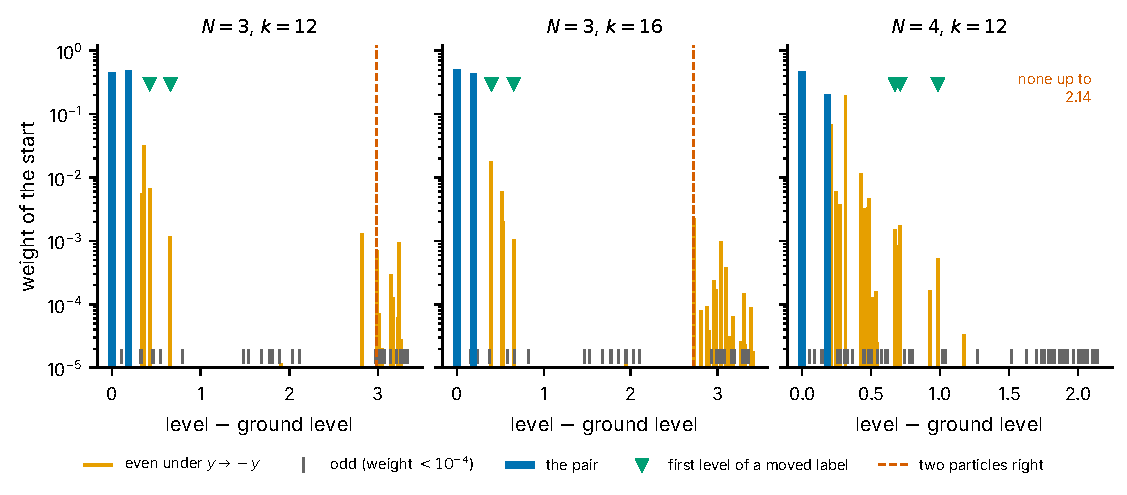
\includegraphics[width=\textwidth]{figures/fig_parity.pdf}
\caption{\textbf{Levels, their reflection parity and the weight of the start.} Lowest levels of $\hat H$ at the resonance tilt, $N=3$ ($k=12,16$) and $N=4$ ($k=12$). Orange: levels even under the reflection $y_i\to-y_i$ of all particles, with the weight of the start on them; grey ticks: odd levels (all carry less than $\num{fu_oddmax_N4_k12}$ of the start). Blue: the pair. Green triangles: the first even level in which particle $1$ (and $2$, $3$) has moved to the right valley instead of particle $0$; at $N=3$ these lie between $\num{fu_marg_lo}$ and $\num{fu_marg_hi}$ times $J$ from the pair. Red dashed: the first even level with two particles on the right; at $N=4$, $k=12$ there is none among the lowest levels computed.}
\label{fig:parity}
\end{figure}

\begin{table}[ht]
\centering
\footnotesize
\caption{The lowest levels of $\hat H$ that carry weight of the start ($N=3$, $k=16$, resonance tilt): energy above the ground state, weight of the start, reflection parity $\langle R\rangle$ and right-valley occupation $\langle n_i\rangle$ of each particle. The pair (levels 0 and 2) is carried mainly by particle $0$; level 1 is odd under the reflection and carries no weight; levels 5 and 9 are the first in which particle $1$, then particle $2$, has moved.}
\label{tab:levels}
\begin{tabular}{rccccccc}
\toprule
level & $E-E_0$ & weight & $\langle R\rangle$ & $\langle n_0\rangle$ & $\langle n_1\rangle$ & $\langle n_2\rangle$ \\
\midrule
0 & 0.000 & 0.5102 & +1.000 & 0.52 & 0.04 & 0.02 \\
1 & 0.157 & 0.0000 & -1.000 & 0.47 & 0.02 & 0.01 \\
2 & 0.191 & 0.4415 & +1.000 & 0.45 & 0.15 & 0.03 \\
5 & 0.396 & 0.0178 & +1.000 & 0.02 & 0.74 & 0.04 \\
9 & 0.652 & 0.0011 & +1.000 & 0.01 & 0.01 & 0.88 \\
\bottomrule
\end{tabular}
\end{table}


\paragraph{The cosine counts} of Fig.~\ref{fig:cosines} come from a greedy pursuit with joint refit of the amplitudes, with the frequency of each new cosine scanned on the residual, applied to the stored signal $\langle\Op\rangle(t)$, $0\le t\le200$; at most eight cosines are tried. They are free fits, not predictions.

\paragraph{Tabulating the observable.} The observable is a function of positions, so $|f'(t)|\le N\|K_x\|$ with $\|K_x\|=\pi^2/(2\Delta x^2)=\num{fu_Kx}$ on the grid of this paper, and $f$ can be tabulated to the allowed error $\varepsilon\|\Op\|$ on about $\num{fu_tab_points}$ points for every $N$. This is the reason no reduction-based hardness statement is possible for the fixed family (Section~\ref{sec:regimeend}).

\paragraph{Reproduction.} Every number and figure of this section is computed from the stored level lists, level files and signal fits by the scripts of the repository; the companion report lists which file feeds which object.

\section{The quantum cost model}
\label{app:quantum}

Each particle's grid state takes $n_p=\num{n_p}$ qubits, and the register adds $\num{b_aux}$ qubits of arithmetic workspace and control. A qubitization step is one query to a selection oracle that costs $C_{\rm sel}=2C_{\rm QFT}+C_W(b)$ T-gates, the cost of two Fourier transforms plus one evaluation of the pair potential at fixed-point precision $b=\num{b_fix}$ bits; the latter dominates, and the total is
$C_{\rm sel}=\num{C_sel}$. The Hamiltonian is written as a linear combination of unitaries with one-norm $\lambda=N\lambda_U+\binom N2\lambda_W$, with $\lambda_U=\num{lam_U}$ (the trap maximum on the grid) and $\lambda_W=V_{\rm cap}=\num{lam_W}$, so that the T-gate count is
\begin{equation}
T_{\rm qub}=\big\lceil\lambda\,\Tobs+\ln(1/\varepsilon)\big\rceil\,C_{\rm sel},\qquad \Tobs=\Tobs(N,\mut)\ \text{of Eq.~\eqref{eq:Tobs} with } g_N=1.
\end{equation}
The product-formula count is a second-order step count $r=\lceil\Tobs\sqrt{\Lambda/\varepsilon}\rceil$ with the commutator sum $\Lambda(N)=N\lambda_1+\binom N2\lambda_2$, $\lambda_2=2\max|\nabla W|^2/m=\num{lam_two}$, times the cost per step. One step applies, for each particle, the kinetic factor (two Fourier transforms and a phase, $2C_{\rm QFT}+n_p$ T-gates) and the trap factor ($n_p$), and, for each pair, the pair potential once per Gaussian in the fit of the capped pair wall, so the cost per step is $N(2C_{\rm QFT}+2n_p)+\binom N2K\,C_W$ with $K=\num{k_gauss}$ Gaussians. Because both counts are linear in $\Tobs$, their ratio does not depend on the mass; its size is set by $\lambda_2$,
the squared slope of the capped pair wall, and it is why the product formula falls out of the window at small $N$.

\paragraph{What the model omits.}
Two terms are omitted at leading order and restored in the ``complete'' edge of Table~\ref{tab:quantum}: the mass dependence of the trap frequency in the semiclassical prefactor of Eq.~\eqref{eq:Tobs} ($\omega\propto m^{-1/2}$ along the mass axis of a fixed trap), and the kinetic one-norm $\lambda_{\rm kin}=\num{lam_kin}/m_{\rm rel}$. Restoring both lowers the edge by $\num{edge_shift_8}$ at $N=8$.
Not modelled: preparation of the correlated start, error-correction overheads beyond the T-gate count, repeated measurements for precision $\varepsilon$ on a bounded observable. The semiclassical form of Eq.~\eqref{eq:Tobs} is an interpolation anchored at the measured
switching time at $\mut_0=\num{mut0}$, not an ab-initio law (Section~\ref{sec:model}).
